%% Doc Props
\documentclass[10pt,a4paper]{report}
\usepackage[utf8]{inputenc}
\usepackage[swedish]{babel}

% Packages
\usepackage{
  titlesec,  textcomp,  fixltx2e,  color,  fullpage,  graphicx,  afterpage,  float,  parskip,  xfrac,  gensymb, verbatim, titlesec,  mathtools, pdfpages, etoolbox, hyperref
}
\usepackage[font={small,it}]{caption} %% Italics in captions


% PDF props
\hypersetup{
  bookmarks=true,              % show bookmarks bar?
  bookmarkstype=toc,
  bookmarksopenlevel=\maxdimen
  unicode=true,                % non-Latin characters in Acrobat’s bookmarks
  pdftoolbar=true,             % show Acrobat’s toolbar?
  pdfmenubar=true,             % show Acrobat’s menu?
  pdffitwindow=false,          % window fit to page when opened
  pdfstartview={FitH},         % fits the width of the page to the window
  pdftitle={Design Specification},         % title
  pdfauthor={Petersson, Oscar}, % author
  pdfsubject={TDDI02},          % subject of the document
  pdfkeywords={TDDI02}          % list of keywords
  pdfnewwindow=true,           % links in new window
  hidelinks,                   % hide links (removing color and border)
  linktocpage=true,
  linktoc=all,                 % parts of TOC made into links
  pdfdisplaydoctitle=true      %display document title instead of file name in title bar
}
\urlstyle{same}

% More Props
\graphicspath{{./fig/}}

% Add Bibliography to ToC
\apptocmd{\thebibliography}{\csname phantomsection\endcsname\addcontentsline{toc}{chapter}{\bibname}}{}{}

% Comfy Command Redefinitions
\newcommand{\bve}{\begin{verbatim}}
\newcommand{\itb}{\begin{itemize}}
\newcommand{\ite}{\end{itemize}}
\newcommand{\tb}{\textbackslash}
\newcommand{\citep}[1]{\emph{Datablad \cite{#1}}}
\renewcommand{\contentsname}{Innehållsförteckning}


%% First Page Information
\author{Matteus Laurent, Johan Levinsson, Oscar Petersson, Erik Peyronsson}
\title{MatLabb - Designspecifikation}
\date{\today}
\newcommand{\course}{Programmeringsprojekt, HT15}
\newcommand{\coursenumber}{TDDI02, Linköpings universitet}
\newcommand{\programme}{Högskoleingenjörsutbildning i datateknik, 180 hp}
\newcommand{\examiner}{Johan Frimodig}
\newcommand{\institution}{Institutionen för datavetenskap}
\newcommand{\reptype}{Designspecifikation}
\newcommand{\Ingredient}{\texttt{Ingredient}}
\newcommand{\InfoIngredient}{\texttt{InfoIngredient}}
\newcommand{\RecipeIngredient}{\texttt{RecipeIngredient}}
\newcommand{\RelatedRecipe}{\texttt{RelatedRecipe}}
\newcommand{\Lookup}{\texttt{Lookup}}
\newcommand{\Recipe}{\texttt{Recipe}}
\newcommand{\Shell}{\texttt{Shell}}
 
 

%\newcommand{\includelogo}{
\includegraphics[width=48 mm]{LiTH_sigill_sv.pdf}\makeatletter\begin{center}\vskip 4.5cm}
\newcommand{\excludelogo}{\makeatletter\begin{center}~\vfill}

%% Remove chapter ``chapter'', keep chapter number
\makeatletter
\renewcommand{\@makechapterhead}[1]{%
  \vspace*{50 pt}%
          {\setlength{\parindent}{0pt} \raggedright \normalfont
            \bfseries\Huge
            \ifnum \value{secnumdepth}>1
            \if@mainmatter\thechapter.\ \fi%
            \fi
            #1\par\nobreak\vspace{40 pt}}}
\makeatother


%%% Document %%%
\begin{document}

\setcounter{secnumdepth}{3}
\setcounter{tocdepth}{3}

%% Custom titlepage, empty backside, do not use with \maketitle
\pagestyle{empty}
%\includelogo
 \excludelogo
  \Large{\@author}\vskip .3cm
  \textbf{\LARGE{\@title}}\vskip .2cm
  \large{\programme}
  \vfill
\end{center}
\reptype{} - \@date\hfill Handledare:\\
\textbf{\course}\hfill\examiner\\
\coursenumber\hfill\institution
\makeatother
\newpage
\afterpage{\null\newpage}
\thispagestyle{empty}

%% Table of Contents
\addtocontents{toc}{\protect\hypertarget{toc}{}}
\tableofcontents\label{sec:toc}
\addtocontents{toc}{\protect\thispagestyle{empty}}
\cleardoublepage

\em Många dokument riktar sig till utvecklare, en sån som du själv. Även om det förstås är viktigt att vara klar och tydlig, fri från motsägelser, och välstrukturerad när man skriver ett sånt har man i alla fall den fördelen att rikta sig till personer med samma bakgrund, och man delar fackkunskap, erfarenheter, terminologi och rent av 'jargong'. Rent språkligt är det därför inte så problematiskt att författa mer 'tekniska' dokument.

När det gäller en manual - användarhandledning - är situationen givetvis en helt annan. Man riktar sig nu till en 'anonym' läsekrets, om vars bakgrund och erfarenheter man inte vet något. Där kan finnas fullständiga noviser, likaväl som mycket väl insatta personer. Detta gör att det är mycket viktigt att lägga sig på 'rätt nivå' både vad gäller språkbruk och 'pedagogik'. Man får vare sig överskatta eller underskatta läsarna! Inte förutsätta att termer och handgrepp är välkända, men inte heller 'för barnsliga'. Inte använda vardagsslarvigt språk, och inte heller 'kanslispråk'. Det här är mycket kinkigt - d.v.s. både viktigt och knepigt!

En användarhandledning är ett dokument som man ska kunna läsa utan att ha programvaran till hands, men ändå i stora drag förstå hur man ska gå tillväga. Det måste ha en god pedagogisk struktur, så att 'kunskaper' och förståelse bygger på varandra. Specifika termer, som man gott kan använda, måste naturligtvis förklaras. Illustrationer är vanligen till god hjälp.

Strukturen på manualen skulle kunna vara denna:

\begin{itemize}
\item Syftet med programvaran - vilket problem vilken uppgift understöder den?
\item Allmän översikt över handhavandet, t.ex. generella principer för interaktionerna.
\item Förteckning över kommandon eller motsvarande: mina handgrepp, systemets responser. Listan kan kanske ha två nivåer - först grundläggande saker, sen lite mer avancerade kommandon, om sådan nivåindelning kan urskiljas.
\item Eventuellt kan man tillfoga en 'how to get started' / 'tutorial', om systemet är någorlunda omfattande. Alltså, en följd av inledande 'åtgärder' i logisk följd, och ganska detaljerat beskrivna, för att lösa ett typiskt problem.
\item En avslutande koncis sammanfattning, en 'snabbreferens' över kommandon (eller motsvarande) kan behövas. Speciellt om det finns många kommandon.
\end{itemize}
\em

%%%%%%%%%%%%%%%%%%%%%%%%

\chapter{Introduktion: MatLabb}
Matlabb är en interaktiv databas för att underlätta
matlagningsprocessen och har hjälpt människor lösa livspusslet sedan
2015. Matlabb erbjuder en rad funktioner för sökning och organisering
av recept, information om pris och näringsinnehåll finns alltid
lätttilgängligt via gränssnittet och ett recept finns alltid max fyra
klick bort.

Matlabb har en rad avancerade filtreringsfunktioner som hjälper dig
att filtrera bort oönskat resultat för att det önskade receptet alltid
skall finnas så nära som möjligt, och äntligen kan alla allergiker
sluta oroa sig, med matlabb går det alltid att filtrera bort recept
som innehåller allergener och användaren slipper själv fundera på om
den kan äta en maträtt eller eller inte.

Detta dokument är en användarhandledning som är tänkt att vara en
referens för användande samt hjälpa användaren komma igång med Matlabb.


\chapter{Översikt, användargränssnitt}
\begin{frame}
  \frametitle{MatLabb}
  \framesubtitle{Översikt}
  \begin{itemize}
    \item MatLabb har tre delsystem:
      \begin{itemize}
        \item GUI -- Det grafiska användargränssnittet
        \item Shell -- Innehåller objekt och variabler
        \item Lookup -- Verktyg för kommunikation med databasen
      \end{itemize}
  \end{itemize}
\end{frame}


\chapter{Använargränssnitt Detaljerad beskrivning}


  \section{Vy 1: Sök}
  När Matlabb startas möts man av Matlabbs hjärta, Sök-vyn. Det är här
användaren söker efter och öppnar recept. Den enkla användaren behöver
bara trycka på \verb+sök+knappen och kan enkelt öppna det recept den är
intresserad av av recepten som dyker upp i listan. Mem det finns två
sätt att söka efter recept i matlabb, Titelsök och Filtersök.


\begin{figure}[h]
        \centering 
        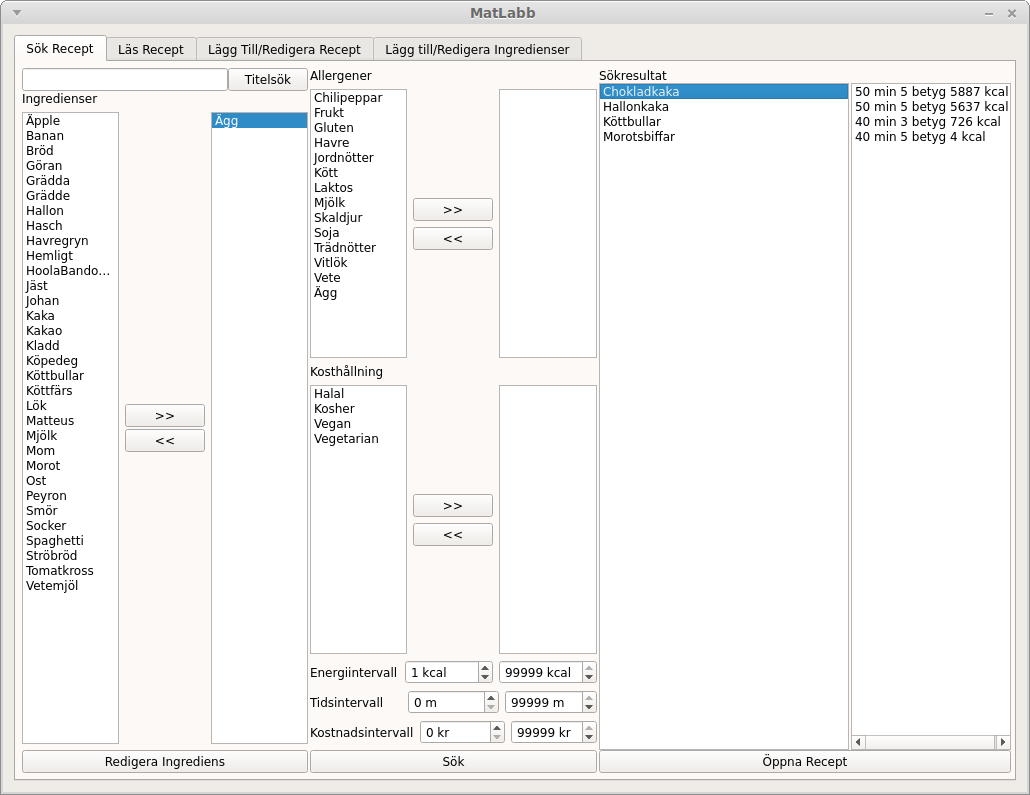
\includegraphics[scale=0.44]{sok_recept.png} 
        \caption{Sökvyn} 
        \label{fig:sokvyn}
\end{figure}


\subsection{Titelsökning}
Vet man redan vilket recept man är ute efter kan det enkelt och snabbt
hittas med hjälp av titelsökfunktionen. Receptets namn matas in i
titelsök rutan och hittas med \verb+titelsök+-knappen och kan sedan öppnas
med knappen \verb+Öppna+. Medans detta räcker för många kan även den
avancerade användaren istället filtrera sina sökningar.

\subsection{Filtersökning}

Matlabb har ett flertal avancerade filtreringsmekanismer, varav den
mest centrala är Ingrediensfiltrering. Ingrediensfiltret finns till
vänster i sök-vyn märkt Ingredienser. För att inkludera en ingrediens
i listan markeras den och flyttas till Sök-listan med hjälp av \verb+>>+
knappen. Vill man ta bort en ingrediens från sök-listan görs detta med
hjälp av \verb+<<+ knappen.

Till höger om Ingreienslistan ses två liknande listor. Genetiska
tillkortakommanden samt kosthållning som används för att filtrera bort
recept innehållande en viss allergen eller ifall man vill exkludera
recept av etiska eller religiösa skäl. Dessa fungerar på precis samma
sätt som för ingrediensfiltrering.

Under kosthållningslistan finns filtren för Energiinnehåll tidsåtgång
och portionskostnad. Filtreringen görs genom att med hjälp av pilarna
ange ett intervall om kommer begränsa sökningen till recept innom
intervallet.

När filtreringsinställningarna är färdiga slutförs sökningen genom att
knappen \verb+Sök+ trycks in och recepten dyker upp i listan till höger. För
att öppna ett recept markeras dess namn och när knappen \verb+öppna+ trycks
in skickas man vidare till recept-vyn.  

%section Receptvyn
I receptvyn möts man av en rad fält. I huvudfältet längst upp finner
man information om receptets namn antal kilokalorier per portion,
antal kronor per portion och hur lång tid receptet tar att laga.

Under huvudfönstret finns från vänster sett Ingrediensfältet,
instruktionsfältet samt kommentarsfältet. I ingrediensfältet finns de
ingredienser som krävs samt åtgångsmängd, i instruktionsfältet finns
instruktioner och i kommentarsfältet finns det möjlighet för korta
kommentarer ifall man inte önskar att ändra receptet.

  \section{Vy 2: Läs recept}
  \begin{figure}[H]
        \centering 
        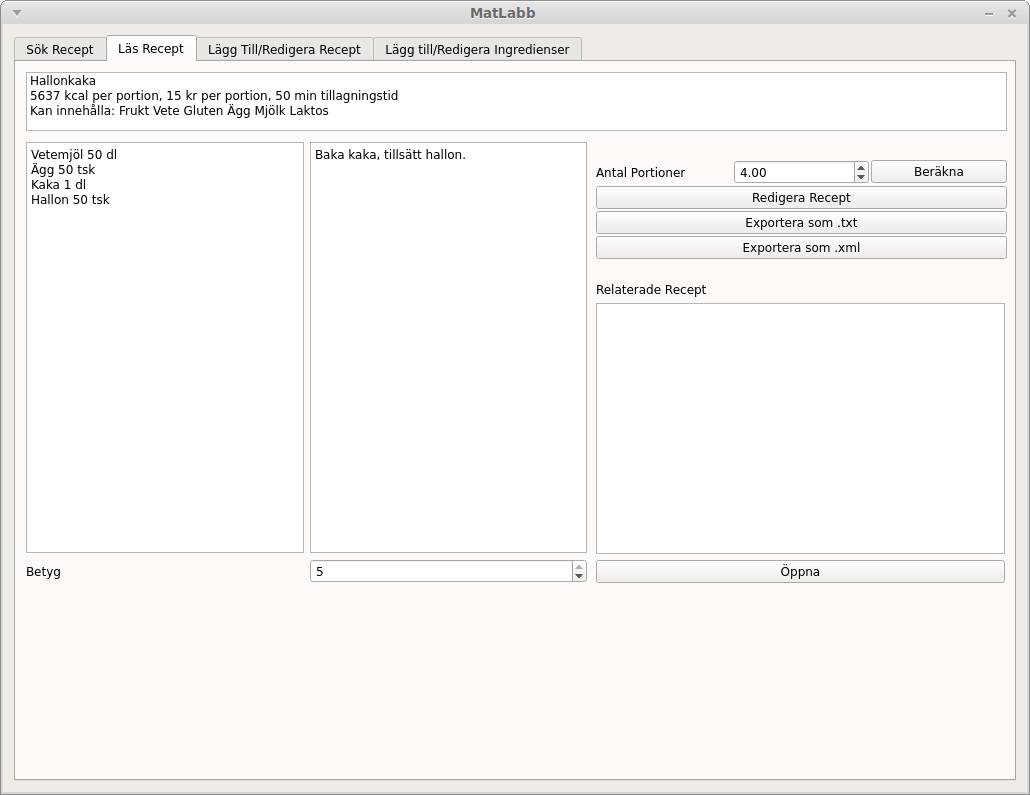
\includegraphics[scale=0.44]{las_recept.png} 
        \caption{Läs receptvyn} 
        \label{fig:receptvyn}
\end{figure}

I \verb+Läs recept+-vyn möts man av en rad fält. I huvudfältet längst upp finner
man information om receptets namn antal kilokalorier per portion,
antal kronor per portion och hur lång tid receptet tar att laga.

Under huvudfönstret finns från vänster sett Ingrediensfältet,
instruktionsfältet samt portionsskalning och knappar för imort/exort
och redigering . I ingrediensfältet finns de ingredienser som krävs
samt åtgångsmängd, i instruktionsfältet hittar man de instruktioner
som behövs för att tillaga maträtten.

Till höger om instruktionsfältet finns portionsskalaren. Med pilarna
kan antalet portioner ändras och när knappen \verb+beräkna+ trycks in
skalas receptet om. Under knapparna för redigering och export finns en
lista över relaterade recept som kan öppnas med knappen \verb+öppna+.

Nederst i fönstret kan receptets betyg öppnas med pilarna.

  \section{Vy 3: Lägg till recept}
  I fliken \verb+Lägg till/Uppdatera recept+ finner du all funktionalitet som har att göra med att lägga till och uppdatera recept. Öppnade du ett befintligt recept så kommer alla fälten att vara ifyllda, redan. De går att redigera genom samma metodik som används för att lägga till recept. För att lägga till ett recept från en extern källa så som en bok följer man följande steg i godtycklig ordning, förutom det allra sista steget som måste ske sist. 

\begin{figure}[H]
        \centering 
        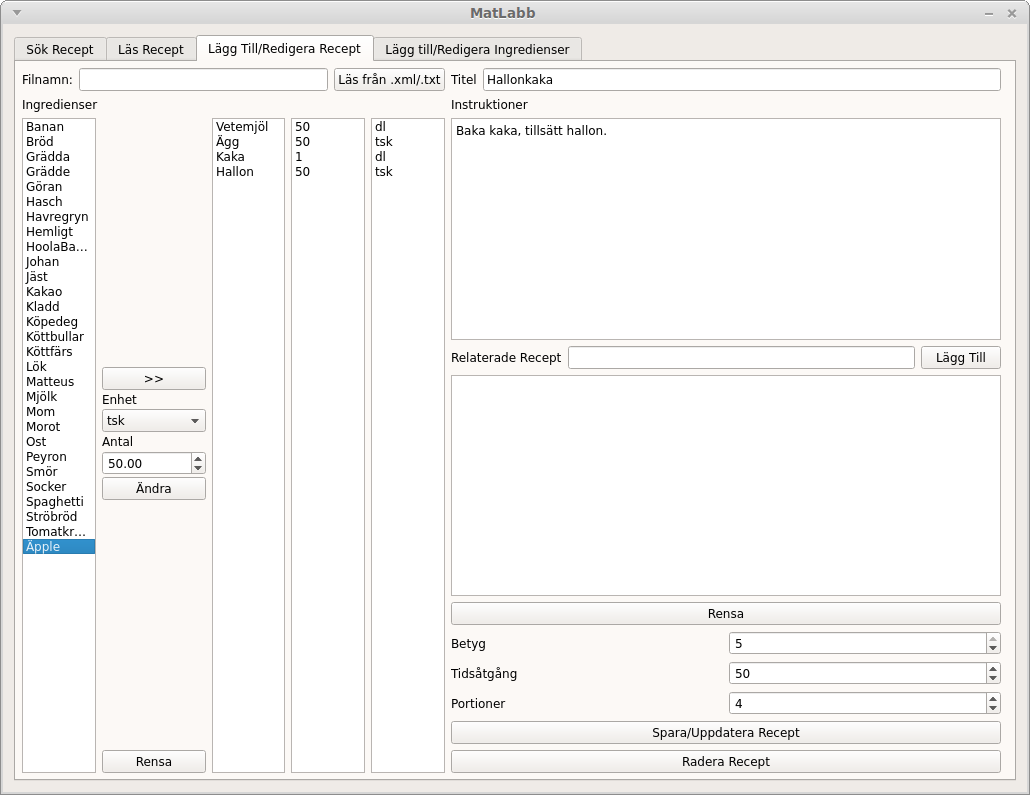
\includegraphics[scale=0.44]{lagg_till_recept.png} 
        \caption{Lägg till/Redigera Recept} 
        \label{fig:laggtillreceptvyn}
\end{figure}

\begin{itemize}
\item Steg 1: Fyll i en titel som är unik för ditt recept. Fyller du i en titel på ett recept som redan finns sparat så kommer detta recept sparas över med ny information.
\item Steg 2: Markera en ingrediens i kollumen till vänster. Ange information om vilken mängd och måttenhet som ingrediensen skall användas i. Klicka sedan på knappen \verb+>>+ för att lägga till ingrediensen i receptet. Upprepa detta tills alla ingredienser som krävs för receptet är angivna .
\em Om misstag sker vid inmatning, exempelvis om man råkar ange fel måttenhet eller mängd kan detta enkelt fixas. Markera ingrediensen i kollumnen med ingredienser, fyll i rätt måttenhet och mängd i fälten mellan kollumnerna, och klicka på knappen \verb+Ändra+. 
Om väldigt många misstag sker vid inmatning, så kan knappen "Rensa" användas för att ta bort alla ingredienser från receptet, då finns möjlighet att börja om från början och försöka göra inmatningen igen. \em
\item Steg 3: Finns det relaterade recept till ditt recept? Fyll då i titlarna i fältet "Relaterade Recept", en efter en, och klicka på knappen \verb+Lägg Till+ emellan. Dessa titlar kommer nu visas i en lista alldeles under fältet. Dessa recept kommer man enkelt att hitta när man sedan öppnar det här receptet. Knappen \verb+Rensa+ tömmer den här listan. 
\item Steg 4: Fyll i ett betyg. Detta kan göras senare då man lagat receptet och vet hur man skulle betygsätta det. 
\item Steg 5: Fyll i uppskattad tidsåtgång.
\item Steg 6: Fyll i hur många portioner som receptet är skrivet till. 
\item Steg 7: Klicka på \verb+Spara/Uppdatera Recept+ receptet finns nu sparat, det går att söka på och öppna. Redigerar du ett existerande experiment så finns nu receptet uppdaterat med ny angiven information.

\em Värt att notera är att recept sparas efter titel. Sparas ett recept med en titel som redan existerar, så kommer det existerande receptet att sparas över. Öppnas ett recept för redigering, och sparas med nytt namn så kommer det existera en gammal version av receptet och en ny version. Knappen \verb+Radera Recept+ raderar det recept som har titeln i titelfältet.\em
\end{itemize}

\subsection{Import av recept från fil}
För att mata in ett recept via .txt eller .xml-fil, så placeras filen i samma map som MatLabb ligger i. Skriv sedan filnamnet i fältet \verb+Filnamn+, och klicka på knappen \verb+Läs från .txt/.xml+. Matlabb kommer då att fylla i alla fält för att lägga till recept baserat på vad som finns i filen. Det återstår då för dig att kontrollera att inläsningen skett korrekt, gör eventuella korrigeringar, och klicka sedan på \verb+Spara/Uppdatera Recept+.

Om du är intresserad att skriva filer som är importerbara av MatLabb så finns det information om detta i appendix.

  \section{Vy 4: Lägg till ingrediens}
  I vyn lägg till ingrediens finner man ett titelfält, en kollumnpar för allergener och ett för kosthållning. Det finns ett fält för kostnad och ett för energiinnehåll. Det är här man sparar ingredienser för att senare använda dem i ett recept.

\begin{figure}[H]
        \centering 
        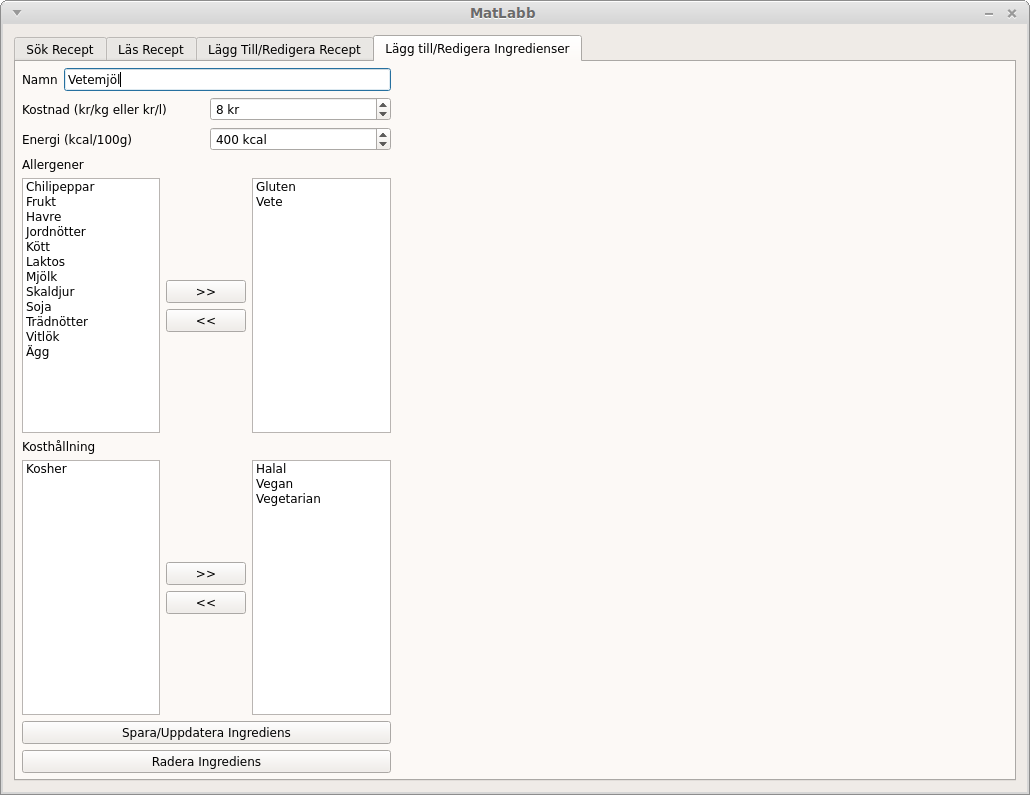
\includegraphics[scale=0.44]{lagg_till_ingrediens.png} 
        \caption{Lägg till/Redigera Ingrediens} 
        \label{fig:laggtillingrediensvyn}
\end{figure} 

Detta görs på följande vis, i godtyckligt ordning, förutom sista steget som måste ske sist. 

\begin{itemize}
\item Steg 1: Fyll i en titel i titelfältet.
\item Steg 2: Fyll i energiinehåll i energifältet.
\item Steg 3: Fyll i kostnad i kostnadsfältet. 
\item Steg 4: Markera de allergener, och klicka på knappen \verb+>>+ för att lägga till dem till ingrediensen. 
\item Steg 5: Markera de kosthållningar som man kan upprätthålla samtidigt som man äter din ingrediens. Lägg till dessa på samma sätt som allergener.
\item Steg 6: Klicka på \verb+Spara/Uppdatera Ingrediens+. Nu går ingrediensen att lägga till i recept och användas för att söka bland recept.
\end{itemize}



  


\end{document}
